%package list
\documentclass{article}
\usepackage{amsmath}
\usepackage[top=3cm, bottom=3cm, outer=3cm, inner=3cm]{geometry}
\usepackage{multicol}
\usepackage{graphicx}
\usepackage{url}
%\usepackage{cite}
\usepackage{hyperref}
\usepackage{array}
%\usepackage{multicol}
\newcolumntype{x}[1]{>{\centering\arraybackslash\hspace{0pt}}p{#1}}
\usepackage{natbib}
\usepackage{pdfpages}
\usepackage{multirow}
\usepackage[normalem]{ulem}
\useunder{\uline}{\ul}{}
\usepackage{svg}
\usepackage{xcolor}
\usepackage{minted}

%\usepackage{booktabs}
\usepackage{caption}
\usepackage{subcaption}
\usepackage{float}
\usepackage{array}

\newcolumntype{M}[1]{>{\centering\arraybackslash}m{#1}}
\newcolumntype{N}{@{}m{0pt}@{}}

%%%%%%%%%%%%%%%%%%%%%%%%%%%%%%%%%%%%%%%%%%%%%%%%%%%%%%%%%%%%%%%%%%%%%%%%%%%%
%%%%%%%%%%%%%%%%%%%%%%%%%%%%%%%%%%%%%%%%%%%%%%%%%%%%%%%%%%%%%%%%%%%%%%%%%%%%
\newcommand{\itemEmail}{ccapatinta@unsa.edu.pe}
\newcommand{\itemStudent}{Capatinta Almanza Camilo B. A.}
\newcommand{\itemCourse}{Lab. Análisis y Diseño de Algoritmos}
\newcommand{\itemCourseCode}{1702231}
\newcommand{\itemSemester}{IV}
\newcommand{\itemUniversity}{Universidad Nacional de San Agustín de Arequipa}
\newcommand{\itemFaculty}{Facultad de Ingeniería de Producción y Servicios}
\newcommand{\itemDepartment}{Departamento Académico de Ingeniería de Sistemas e Informática}
\newcommand{\itemSchool}{Escuela Profesional de Ingeniería de Sistemas}
\newcommand{\itemAcademic}{2026 - B}
\newcommand{\itemInput}{29/10/2026}
\newcommand{\itemOutput}{02/11/2026}
\newcommand{\itemPracticeNumber}{07}
\newcommand{\itemTheme}{Programación Dinámica: Mochila 0/1 y Mochila Ilimitada}
%%%%%%%%%%%%%%%%%%%%%%%%%%%%%%%%%%%%%%%%%%%%%%%%%%%%%%%%%%%%%%%%%%%%%%%%%%%%
%%%%%%%%%%%%%%%%%%%%%%%%%%%%%%%%%%%%%%%%%%%%%%%%%%%%%%%%%%%%%%%%%%%%%%%%%%%%

\usepackage[english,spanish]{babel}
\usepackage[utf8]{inputenc}
\AtBeginDocument{\selectlanguage{spanish}}
\renewcommand{\figurename}{Figura}
\renewcommand{\refname}{Referencias}
\renewcommand{\tablename}{Tabla} %esto no funciona cuando se usa babel
\AtBeginDocument{%
	\renewcommand\tablename{Tabla}
}

\usepackage{fancyhdr}
\pagestyle{fancy}
\fancyhf{}
\setlength{\headheight}{40.51407pt}
\renewcommand{\headrulewidth}{1pt}
\renewcommand{\footrulewidth}{1pt}
\fancyhead[L]{\raisebox{-0.2\height}{
\includegraphics[width=3cm]{../img/logo_episunsa.png}}}
\fancyhead[C]{\fontsize{7}{7}\selectfont	\itemUniversity \\ \itemFaculty \\ \itemDepartment \\ \itemSchool \\ \textbf{\itemCourse}}
\fancyhead[R]{\raisebox{-0.2\height}{
\includegraphics[width=1.2cm]{../img/logo_abet}}}
\fancyfoot[L]{Estudiante Capatinta C.}
\fancyfoot[C]{\itemCourse}
\fancyfoot[R]{Página \thepage}

% para el codigo fuente

\usepackage{color, colortbl}
\definecolor{dkgreen}{rgb}{0,0.6,0}
\definecolor{gray}{rgb}{0.5,0.5,0.5}
\definecolor{mauve}{rgb}{0.58,0,0.82}
\definecolor{codebackground}{rgb}{0.95, 0.95, 0.92}
\setminted{%
  fontsize=\small,
  breaklines,
  breakanywhere,
  linenos,
  numbersep=6pt,
  frame=lines,
  framesep=3mm,
  baselinestretch=1,
  bgcolor=codebackground,
  tabsize=3
}
\definecolor{tablebackground}{rgb}{0.8, 0, 0}

\begin{document}
	
	\vspace*{10px}
	
	\begin{center}
		\parbox{0.8\textwidth}{\centering\fontsize{17}{20}\selectfont\textbf{Informe de laboratorio \itemPracticeNumber}}
	\end{center}
	\begin{center}
		\parbox{0.8\textwidth}{\centering\textbf{\Large Tema: \itemTheme}}
	\end{center}
	%\vspace*{0.5cm}	

	\begin{flushright}
		\begin{tabular}{|M{2.5cm}|N|}
			\hline 
			\rowcolor{tablebackground}
			\color{white} \textbf{Nota}  \\
			\hline 
			     \\[30pt]
			\hline 			
		\end{tabular}
	\end{flushright}	

	\begin{table}[h!]
		\begin{tabular}{|x{4.7cm}|x{4.8cm}|x{4.8cm}|}        
			\hline 
			\rowcolor{tablebackground}
			\color{white} \textbf{Estudiante} & \color{white}\textbf{Escuela}  & \color{white}\textbf{Asignatura}   \\
			\hline 
			{\itemStudent \par \itemEmail} & \itemSchool & {\itemCourse \par Semestre: \itemSemester \par Código: \itemCourseCode}     \\
			\hline 			
		\end{tabular}
	\end{table}		
	
	\begin{table}[H]
		\begin{tabular}{|x{4.7cm}|x{4.8cm}|x{4.8cm}|}
			\hline 
			\rowcolor{tablebackground}
			\color{white}\textbf{Laboratorio} & \color{white}\textbf{Tema}  & \color{white}\textbf{Duración}   \\
			\hline 
			\itemPracticeNumber & \itemTheme & 02 horas   \\
			\hline 
		\end{tabular}
	\end{table}
	
	\begin{table}[H]
		\begin{tabular}{|x{4.7cm}|x{4.8cm}|x{4.8cm}|}
			\hline 
			\rowcolor{tablebackground}
			\color{white}\textbf{Semestre académico} & \color{white}\textbf{Fecha de inicio}  & \color{white}\textbf{Fecha de entrega}   \\
			\hline 
			\itemAcademic & \itemInput &  \itemOutput  \\
			\hline 
		\end{tabular}
	\end{table}
	
\section{Ejercicios/Problemas propuestos}

\subsection{Ejercicio 1}

Implementa Mochila 0/1 para un conjunto de al menos 8 objetos ingresados por el usuario e imprime tanto el valor máximo como la lista de objetos elegidos.

\inputminted{cpp}{../e-n/e1.cpp}

\begin{itemize}
    \item En este ejercicio se lee la capacidad de la mochila y los objetos con validación de entrada, y la tabla \texttt{dp[i][w]} guarda el mayor valor alcanzable usando los primeros \textit{i} objetos con capacidad \textit{w}. La transición compara no tomar el objeto contra tomarlo si cabe, y la reconstrucción recorre la tabla desde \texttt{dp[n][W]} hacia arriba para devolver la lista de elementos elegidos con su peso y valor totales. Así, el programa no solo obtiene el valor máximo, sino que también ofrece una verificación clara de que la solución cumple la restricción de capacidad.
\end{itemize}

\begin{figure}[H]
    \centering
    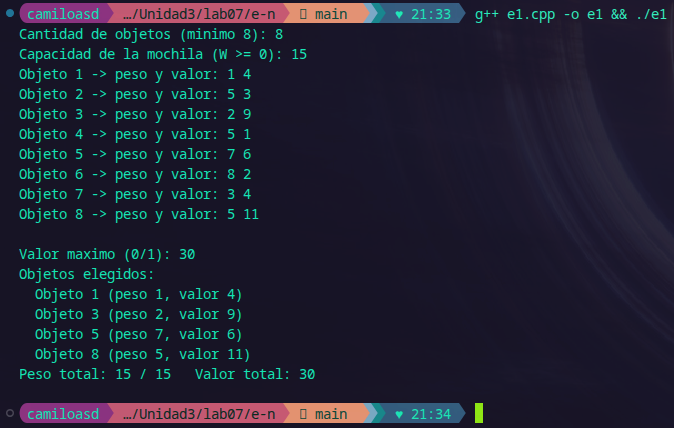
\includegraphics[width=0.8\textwidth]{../img/e1.png}
    \caption{Ejecución del ejercicio 1}
    \label{fig:e1}
\end{figure}

\subsection{Ejercicio 2}

Implementa Mochila Ilimitada para el clásico «problema del cambio de monedas»: dado un conjunto de denominaciones y un monto objetivo, encuentra la combinación que usa la menor cantidad de monedas.

\inputminted{cpp}{../e-n/e2.cpp}

\begin{itemize}
    \item Este problema se modela como una mochila ilimitada: el monto objetivo es la capacidad, cada denominación es un peso y la decisión consiste en usar una moneda o no, con la diferencia de que la misma moneda puede repetirse tantas veces como sea necesario. El arreglo \texttt{dp[m]} guarda el mínimo número de monedas para formar el monto \textit{m}, y la actualización prueba todas las denominaciones con la recurrencia \texttt{1 + dp[m-c]} para conservar la mejor opción. La reconstrucción sigue desde el monto final hasta cero usando la decisión guardada en cada paso, de modo que el programa devuelve la combinación exacta y detecta también cuando un monto es imposible.
\end{itemize}

\begin{figure}[H]
    \centering
    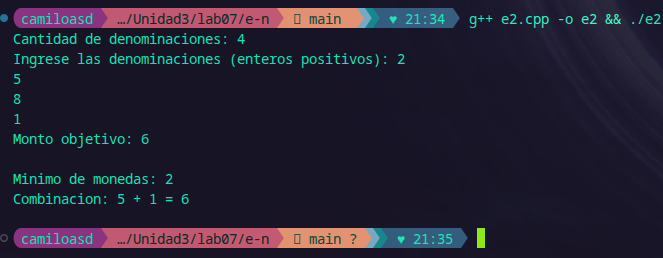
\includegraphics[width=0.8\textwidth]{../img/e2.png}
    \caption{Ejecución del ejercicio 2}
    \label{fig:e2}
\end{figure}

\subsection{Ejercicio 3}

Modifica la solución de Mochila 0/1 para que, además del valor máximo, muestre la tabla `dp` completa (todas las filas y columnas) y explique cómo se reconstruyó la solución.

\inputminted{cpp}{../e-n/e3.cpp}

\begin{itemize}
    \item La diferencia clave de este ejercicio es que la tabla \texttt{dp} se imprime completa para que el lector observe la evolución del algoritmo en cada fila y columna. Cada celda compara la opción de no tomar el objeto con la de tomarlo si cabe, y la reconstrucción explica el porqué de cada decisión observando si \texttt{dp[i][w]} cambia respecto a \texttt{dp[i-1][w]}. Esto permite visualizar, de manera didáctica, cómo se obtiene el valor máximo y qué objetos forman la solución final sin perder la lógica de programación dinámica.
\end{itemize}

\begin{figure}[H]
    \centering
    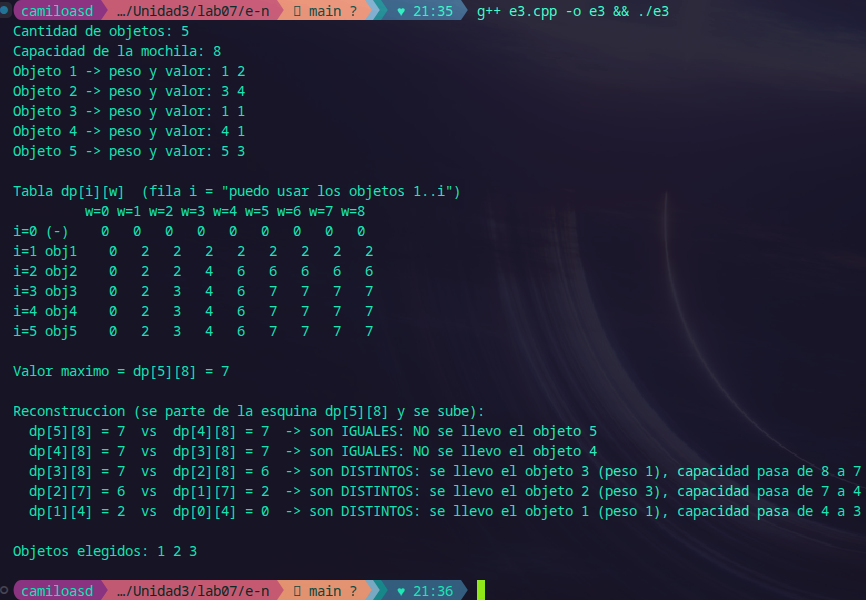
\includegraphics[width=0.8\textwidth]{../img/e3.png}
    \caption{Ejecución del ejercicio 3}
    \label{fig:e3}
\end{figure}

\subsection{Ejercicio 4}

Compara el uso de memoria de Mochila 0/1 (tabla 2D) contra una versión optimizada que use solo un arreglo 1D recorrido de derecha a izquierda. Explica por qué ese recorrido evita reutilizar el mismo objeto más de una vez.

\inputminted{cpp}{../e-n/e4.cpp}

\begin{itemize}
    \item Aquí se compara la versión 2D, que guarda toda la tabla y permite reconstruir la solución, con la versión optimizada en 1D que usa un solo arreglo para reducir la memoria a \textit{O(W)}. La clave está en recorrer la capacidad de derecha a izquierda, porque así la posición \texttt{dp[w - peso]} aún conserva el valor de la fila anterior y no se reutiliza el mismo objeto en la misma pasada. Si se recorre de izquierda a derecha, la celda ya queda actualizada con el mismo objeto y la solución se comporta como una mochila ilimitada; el programa demuestra exactamente esta diferencia y la comparación de memoria entre ambas versiones.
\end{itemize}

\begin{figure}[H]
    \centering
    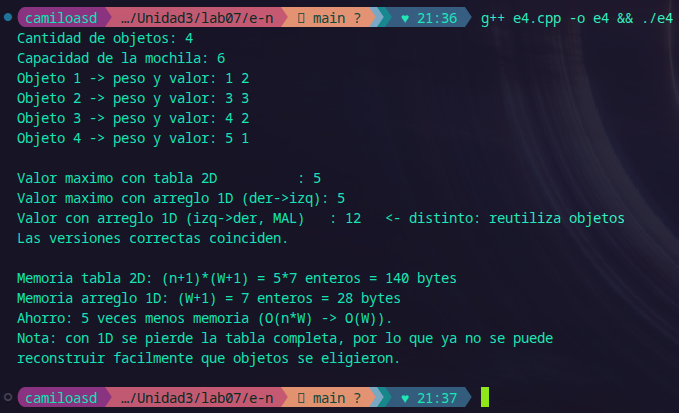
\includegraphics[width=0.8\textwidth]{../img/e4.png}
    \caption{Ejecución del ejercicio 4}
    \label{fig:e4}
\end{figure}

\subsection{Ejercicio 5}

Aplica Mochila 0/1 a un caso real: dado un presupuesto fijo y una lista de posibles compras (con costo y beneficio estimado), determina la combinación que maximiza el beneficio sin exceder el presupuesto.

\inputminted{cpp}{../e-n/e5.cpp}

\begin{itemize}
    \item En este caso cada compra se convierte en un objeto con peso igual al costo y valor igual al beneficio estimado, mientras que el presupuesto representa la capacidad de la mochila. La tabla \texttt{dp} calcula el mejor beneficio posible para cada nivel de gasto disponible y, luego, la reconstrucción vuelve hacia atrás para elegir exactamente las compras que forman el plan óptimo. La salida final incluye el nombre, costo, beneficio, gasto total y sobrante, por lo que la solución no solo maximiza el valor, sino que además queda validada frente al presupuesto real.
\end{itemize}

\begin{figure}[H]
    \centering
    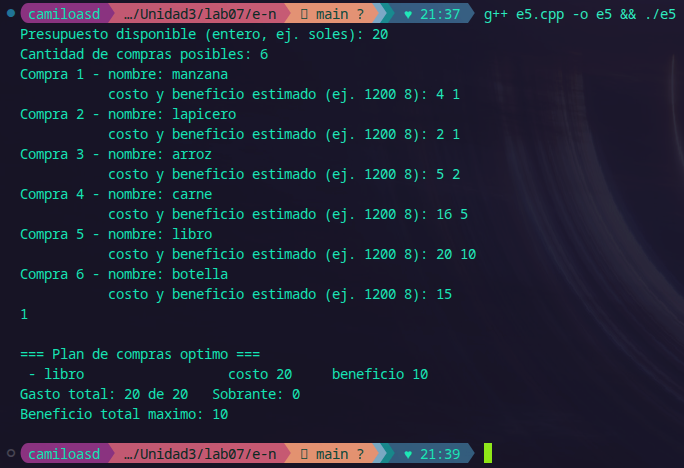
\includegraphics[width=0.8\textwidth]{../img/e5.png}
    \caption{Ejecución del ejercicio 5}
    \label{fig:e5}
\end{figure}

\section{Cuestionario}
\begin{enumerate}
    \item ¿Por qué Mochila 0/1 necesita una tabla bidimensional, mientras que Mochila Ilimitada se resuelve con un arreglo unidimensional? \\ 
    Porque en Mochila 0/1 cada objeto puede elegirse o no elegirlo una sola vez, por lo que el estado debe recordar qué objetos ya fueron considerados; por eso se requiere la dimensión \texttt{i} para distinguir entre los primeros \textit{i} objetos y la dimensión \texttt{w} para la capacidad restante. En la versión ilimitada, la misma moneda u objeto puede reutilizarse, así que solo basta recordar el mejor valor para cada capacidad, lo que se representa con un solo arreglo \texttt{dp[w]}.

    \item En Mochila 0/1, ¿qué representa exactamente el valor \texttt{dp[i][w]}? \\ 
    Representa el máximo beneficio (o valor) que se puede obtener usando solo los primeros \textit{i} objetos y una capacidad total de \textit{w}. Es decir, es el mejor resultado posible para ese subproblema, sin exceder la capacidad disponible.

    \item ¿Por qué en el ejemplo resuelto Mochila Ilimitada obtiene un valor mayor que Mochila 0/1 con la misma capacidad? \\ 
    Porque en Mochila Ilimitada un mismo elemento puede aparecer varias veces, mientras que en Mochila 0/1 cada objeto se toma a lo más una vez. Por ello, la versión ilimitada puede repetir una denominación o una compra, lo que permite acumular más valor o formar montos más grandes con la misma capacidad.

    \item ¿Cómo se podría adaptar Mochila 0/1 para permitir llevar cada objeto hasta un número limitado de veces (por ejemplo, máximo 3 unidades de cada uno)? \\ 
    Se puede extender el estado con una tercera dimensión que indique cuántas copias del objeto actual ya se han usado. En la práctica, para cada objeto \textit{i} y cada capacidad \textit{w}, se prueba si se toman 0, 1, 2 o 3 unidades del mismo elemento, y se actualiza la tabla usando el valor correspondiente. También se puede convertir este problema en un caso de mochila con multiplicidad limitada, donde el objeto tiene varias versiones de copia.

    \item ¿Qué papel cumple el paso B (casos base) de SRTBOT en ambas variantes de la mochila? \\ 
    El caso base define los estados iniciales del problema: cuando no hay objetos disponibles o la capacidad es cero, el valor máximo es cero. Esto evita decisiones ambiguas y garantiza que la recurrencia comience desde una base correcta; en la mochila ilimitada, además, se inicializa \texttt{dp[0] = 0} y los demás estados con infinito si son imposibles.
\end{enumerate}

\section{Conclusiones}

La programación dinámica fue la herramienta clave para resolver los problemas planteados porque permite dividir un problema complejo en subproblemas más pequeños y reutilizar resultados ya calculados. En la mochila 0/1 y en la mochila ilimitada, la estructura recursiva permite decidir si conviene incluir o excluir un elemento sin perder la optimización global, y la tabla \texttt{dp} refleja exactamente ese proceso.

Durante el laboratorio se observó que la diferencia entre ambas variantes no está solo en la fórmula, sino en la interpretación del estado: en mochila 0/1 cada objeto se considera una sola vez, mientras que en la versión ilimitada se permite reutilizarlo con el mismo costo de una nueva elección. Esta diferencia cambia completamente la forma de recorrer la tabla y la complejidad práctica de la solución.

Además, los ejercicios demostraron que la programación dinámica no solo resuelve el valor óptimo, sino que también permite reconstruir la solución final, algo esencial cuando se desea mostrar qué objetos o compras forman la mejor elección. En conjunto, la práctica mostró que esta técnica es útil no solo en teoría, sino también en aplicaciones reales como la planificación de compras, el cambio de monedas y la optimización de recursos.

	%\begin{itemize}	
	%	\item Se creo el archivo \textbf{.gitignore} para no considerar los archivos %\textbf{*.class} que son innecesarios hacer seguimiento.
	%\end{itemize}
	%\begin{lstlisting}[language=bash]
	%	$ vim lab01/.gitignore
	%\end{lstlisting}
	%\begin{lstlisting}[language=bash]
	%	*.class
	%\end{lstlisting}
	%\begin{lstlisting}[language=bash]
	%	$ git add .
	%	$ git commit -m "Creando .gitignore para archivos *.class"			
	%	$ git push -u origin main
	%\end{lstlisting}
	
	%\begin{lstlisting}[language=bash]
	%	$ vim lab01/Insertion.java
	%\end{lstlisting}
	
    
%\clearpage
%\bibliographystyle{apalike}
%\bibliographystyle{IEEEtranN}
%\bibliography{bibliography}
			
\end{document}\noindent\textbf{Enunciado:}
